\section{ХОД РАБОТЫ}

\subsection{Постановка задачи}

Изготовление некоторых изделий включает сборку (закрепление восьми деталей на плате)
и установку платы в корпус.

Детали поступают на рабочее место для сборки партиями по 40 шт.
Интервалы между моментами поступления партий --- случайные величины,
распределенные по экспоненциальному закону, со средним значением 1 час.

Платы поступают по одной; интервалы между моментами поступления плат --- случайные величины,
распределенные по экспоненциальному закону, со средним значением 10 мин.

Время закрепления одной детали на плате --- случайная величина, 
распределенная по гауссовскому закону, со средним значением 3 мин и стандартным отклонением 30 с.
Закрепление деталей на плате начинается только тогда, когда на рабочем месте для сборки
имеется восемь деталей и плата.

Собранные платы направляются на рабочее место для установки в корпуса.
Корпуса поступают на это место партиями по 10 штук; интервалы между моментами поступления корпусов
--- случайные величины, распределенные по экспоненциальному закону, со средним значением 10 мин.
Установка платы в корпус занимает от 2 до 5 мин.

Требуется разработать GPSS-модель для анализа процесса выпуска изделий в течение 100 часов.
Предусмотреть подсчёт количества выпущенных готовых изделий.

\subsection{Решение задачи}

Разработанная GPSS-модель представлена в приложении~А. После выполнения сеанса
моделирования исходной задачи, получим отчёт, представленные на
рисунках~\ref{pic:report_1}--\ref{pic:report_2}.

\begin{figure}[h!]
  \centering
  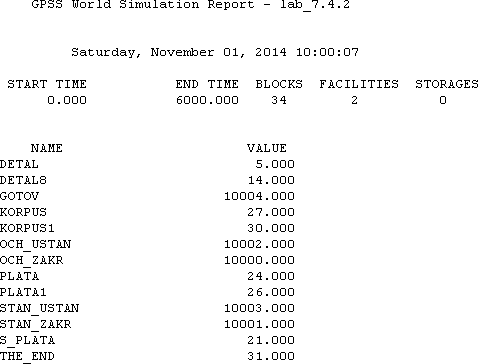
\includegraphics[width=0.8\linewidth]{pic/report_1}
  \caption{Выходные данные имитационной модели}
  \label{pic:report_1}
\end{figure}

\begin{figure}[h!]
  \centering
  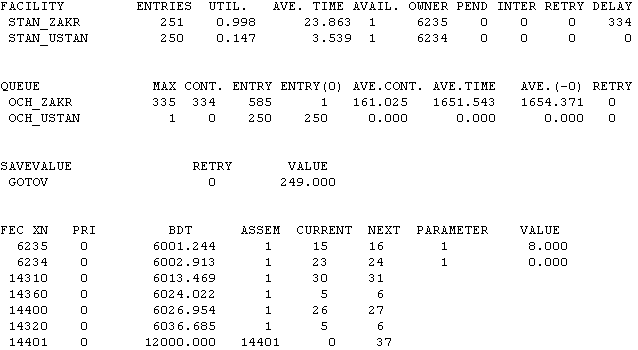
\includegraphics[width=1\linewidth]{pic/report_3}
  \caption{Статистика использования узлов моделируемой СМО}
  \label{pic:report_stat}
\end{figure}

Общее число выпущенных изделий хранится в переменной GOTOV и 
по истечении 100 часов моделирования равно 186.

Исходя из результатов моделирования, можно утверждать, что 
станок, производящий закрепление детали на плате, сильно перегружен,
так как его коэффициент загрузки составляет 0{,}998.

\begin{figure}[h!]
  \centering
  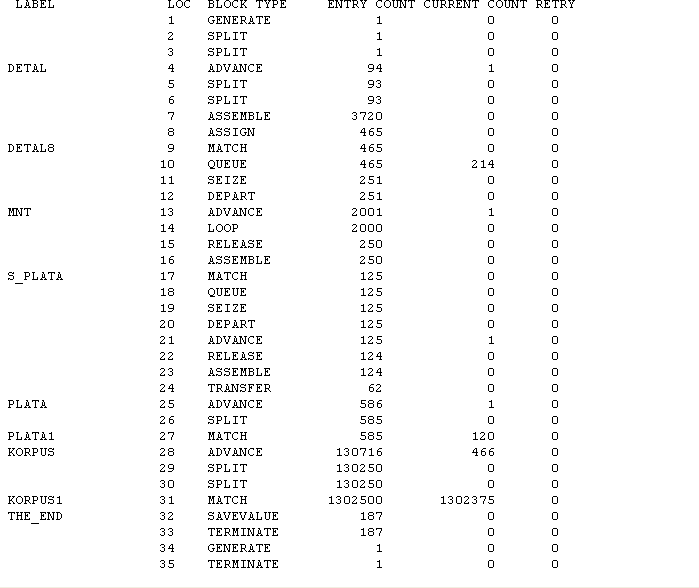
\includegraphics[width=0.8\linewidth]{pic/report_2}
  \caption{Статистика исполнения команд имитационной модели}
  \label{pic:report_2}
\end{figure}


\newpage
